\documentclass[../main-v1.tex]{subfiles}
\begin{document}
\chapter{Computing Organization\hideme{Ready 3/13}}\label{ch:org}

The offline computing organization for DUNE has several facets. The main focus of the formal Computing Consortium (and this document) is the computing infrastructure that allows development and implementation of algorithms and data analysis techniques rather than the algorithms and analysis themselves. Algorithms and analysis are the purview of the physics groups.

Within the Computing organization itself, there are three major subgroups.  There are groups actively engaged in the development of \dword{dune} computing infrastructure, there are groups that are engaged in \dword{dune} specific operations such as the production group and there are a large number of global institutions and sites that contribute computing resources through \dword{osg} and \dword{wlcg} mechanisms.  

This section describes the formal Computing Consortium that concentrates on development and operations for \dword{dune} while chapter \ref{ch:cm} includes a description of the global sites and their hardware contributions. The Computing Consortium and the global sites meet weekly via teleconference to coordinate operations. 

\begin{dunefigure}
[Computing Consortium Organization Chart]
{fig:orgchart}
{DUNE Computing Consortium organization chart, February 2022.}
{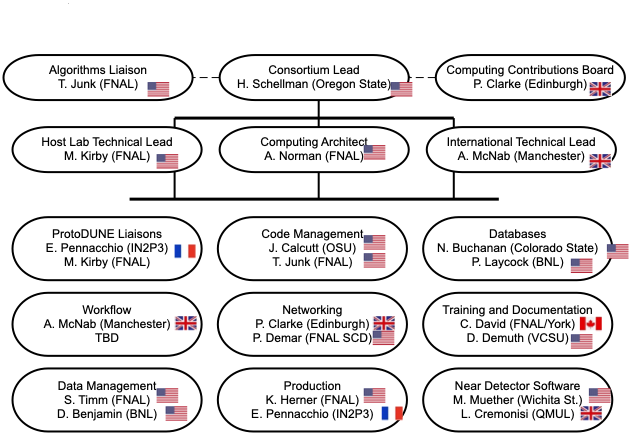
\includegraphics[width=0.9\textwidth]{graphics/IntroFigures/MTOrgChartFeb22.png}}
\end{dunefigure}

Figure \ref{fig:orgchart} shows the Computing Consortium organization as of February 2022.  The Consortium leadership consists of a Consortium Lead, responsible for overall coordination, two technical leads, one US-based and the other from the international collaboration and a Computing Architect.  There is an Algorithms Liaison responsible for coordinating with the Physics group and an independent Computing Contributions Board described in Section \ref{sec:ccb} that negotiates resource contributions from global collaborators. 

The Computing Consortium is not formally part of the \dword{dune} construction project but has representation on the Executive Board.  The Computing Consortium is part of the interface document matrix with the construction consortia and interface agreements exist in the CERN EDMS \cite{dune-edms} system and are listed in Table \ref{tab:intro:interfacedocs}. The most important interfaces are 1) data-management and networking with the DAQ and calibration groups and 2) databases with the DAQ and hardware construction groups. 

\begin{dunetable}
[Interface documents with hardware consortia]
{l l}
{tab:intro:interfacedocs}
{Offline computing \dword{edms} interface documents with hardware consortia. }
Document title&EDMS ID\\
JT COM and SP APA Consortium Interface Document	&2145145 v.4\\
%		
JT COM and SP PD Consortium Interface Document	&2145146	v.2\\
%12		
JT COM and SP TPC Consortium Interface Document	&2145147	v.2\\
%12		
JT COM and DP CRP Consortium Interface Document	&2145148	v.1\\
%17		
JT COM and DP PDS Consortium Interface Document	&2145149	v.1\\
%17		
JT COM and JT HV Consortium Interface Document	&2145150	v.2\\
JT COM and JT DAQ Consortium Interface Document	&2145151	v.2\\
%12		
JT CAL/CI and JT COM Consortium Interface Document	&2145159	v.2\\ 
%12		
JT COM to Facility Interface	&2145167	v.1 \\
\end{dunetable}


\section{Internal organization}

Within the Consortium there are specific development groups responsible for particular components of the computing infrastructure.  Many of these activities are described in greater detail in separate chapters. 

\begin{itemize} 
%ST fixed sp Liaisons
\item ProtoDUNE Liaisons - make certain that offline computing is coordinated with ProtoDUNE data taking and analysis.

\item Data Management - responsible for storage, cataloging and delivery of data. See Chapter \ref{ch:datamgmt}

\item Workflow - responsible for global coordination of CPU and data delivery. See Chapter \ref{ch:wkflow}.


\item Code Management - responsible for maintaining the code infrastructure and  repositories and building common executables.  See Chapter \ref{ch:codemgmt}.

\item{Networking} -  Responsible for negotiating suitable networking capabilities from \dword{surf} to the host laboratories and from the host laboratories to the global compute resources.  See Chapter \ref{ch:netw}. 

\item{Production} - Responsible for setting up and running large reconstruction and simulations jobs. This group includes both experts and collaboration volunteers who run the jobs. See Chapter \ref{sec:current} for a description of the current status. 


\item{Databases} - Responsible for the design and implementation of databases to support offline data processing. See Chapter \ref{ch:db}.

\item{Training, Document and User support} - Responsible for development of training materials, infrastructure for and review of documentation and for directing users to experts and documentation where needed. See Chapter \ref{ch:train}.

\item Near Detector Software - responsible for coordination of the unique \dword{nd} software and integration with the main \dword{dune} infrastructure. See Section \ref{ch:use:nd}. 

\end{itemize}

\section{Funding Sources for Computing Development}
Most personnel working on \dword{dune} computing are supported by their institutions or national funding agencies as part of general or \dword{dune} project support.  One exceptions are a US \dword{doe} funded consortium of 4 universities and 3 national labs funded specifically for \dword{dune} computing infrastructure at a level of \$1M/year, directly supporting postdocs and lab physicists summing to $\sim 6$ FTE.  The UK,  France and CERN also make significant contributions to software development through the DUNE project while many nations contribute substantial hardware capabilities. 


\section{Computing Contributions Board }\label{sec:ccb}

In addition to the formal Consortium, CPU and storage resources are contributed by sites and countries through formal pledges facilitated by the \dword{ccb}. 

The \dword{ccb} has been set up to formalize the contribution of DUNE partners to the computing and storage capacity required for computing production. In order to remain scale-able, the \dword{ccb} considers a nation as the natural unit of aggregation to request and then seek pledges for resources. The \dword{ccb} does, however, recognize that whilst within some countries centralized coordination is natural, this is not true for others. Nevertheless, requests will be published at a national granularity, with the assumption that Institutes within each nation can coordinate.

In order to set a fair-share request for computing capacity, the \dword{ccb} will eventually use a proxy metric for the relative proportion of each nation in DUNE. This is likely to be PhD paper authors once in the exploitation phase. This is, however, not relevant during construction as the current listing of DUNE members in the data base is a very poor proxy for this. Therefore, during construction all nations with more than a minimum number of DUNE participants or providing Tier-1 or large Tier-2 capacity to LHC experiments, are asked to provide a "reasonable" share (see below). We refer to these as compute-active-nations.
This is very flexible and is up to each nation to decide if it wishes to be classified as a compute-active-nation.

At present the \dword{ccb} is composed of a Chair, one member per compute-active-nation, one member for each of FNAL, CERN and BNL, and the Computing and Software Consortium  Management ex officio.

The Computing Consortium management produces an overall requirements document that should be scrutinized by the FNAL CRSG. The \dword{ccb} receives this document, and then seek pledges to meet those requirements. As host lab, FNAL plans to provide ~25\% of the capacity, including the primary tape service.
CERN also currently provides a substantive capacity, in particular for \dword{protodune}.
The aim is then for the remaining capacity to come from other contributors according to the prevailing computing model. A substantial proportion of capacity is expected from outside of the USA  (~50\%). Contributions of at least 5-20\% are requested depending upon the circumstance and capability of each compute-active-nation.
Pledges of capacity received are recorded in the CRIC information system. In due course this process could be formalized into a (non-binding) MOU.

The \dword{ccb} may also receive requests and information from the Computing Consortium Management in respect of any other non-capacity matter. The \dword{ccb} may seek to help with such requests where they pertain to national contributions. This may include promotion of requests for software engineering support to be propagated within each nation.  

Chapter \ref{ch:cm:intro} describes the impact of  collaboration contributions in more detail. 

% \hideme{I propose moving the subsections here into the appropriate later chapters and using this section to describe the global compute model}

% \dword{dune} is a global collaboration with contributions from institutions worldwide.  The large scale computing effort relies on multi-national contributions. The overall strategy for computing resources is for primary raw data storage to reside at the large host labs (CERN and FNAL) with computing resources such as disk and CPU largely contributed by collaborating countries.   CPU contributions are provided by a large number of sites worldwide while storage is concentrated at a few larger international sites. Table \ref{tab:coop:disk} shows the distribution of disk space pledges for 2021 and 2022 while Tables \ref{tab:coop:sites} and \ref{tab:coop:ussites}shows the sites contributing CPU resources. 

% The large LHC experiments have historically relied on a tiered structure, with national Tier-1 centers serving regional Tier-2 and Tier-3 centers.  The DUNE model builds on the emergence of faster networks to move to  a service-oriented model, where sites provide services, disk, CPU, real memory/core and archival tape, and projects are  distributed to them based on their capabilities and available networking.  For example, a site with large CPU and memory/core but slower networking would be ideal for simulation while small memory/core and fast access to large local disk stores would be ideal for high level data analysis.  This model requires a high level view of data locations and job placement with continual monitoring for bottlenecks but allows new sites to contribute in an optimal way. 

% This model builds on the highly successful tools developed by the WLCG and OSG for LHC computing.  As DUNE's needs are substantially smaller that those of the large LHC experiments we can be confident that the existing infrastructure can be incrementally augmented to meet DUNE's requirements. 


% \begin{dunetable}
% [National Disk pledges]{llrr}{tab:coop:disk}
% {Disk pledges in PB for 2021 and 2022 .}
% Country/Lab	&	Name	&	2021	&	2022	\\
% FNAL	&	FNAL	&	2.2	&	7.6	\\
% CERN	&	CERN	&	2.2	&	1.6	\\
% BNL	&	BNL	&	0.5	&	0.5	\\
% UK	&	GridPP	&	4.0	&	4.0	\\
% FR	&	CC-IN2P3	&	0.5	&	0.5	\\
% ES	&	PIC Tier-1	&	0.5	&	0.72	\\
% NL	&	NL/LHC Tier-1	&	1.9	&	1.8	\\
% CZ	&	CZ-Prague-T2	&	0.3	&	1.0	\\
% %BR	&	CBPF	&	0	&		\\
% IN	&	TIFR	&	0.75&	0.75\\
% RU	&	JINR	&	-	&	0.5	\\
% \hline
% Total pledge	&		&	12.85	&	18.97	\\
% \end{dunetable}

% %\tiny
% \begin{dunetable}
% [List of DUNE Compute Sites]
% {l l r l}{tab:coop:sites}
% {List of non-US international DUNE compute sites as of December 2021.  Sites with substantial rucio controlled disk are noted.}
% Site name	&	RC Site	&	Disk	&	Country	\\
% \hline
% BR\_CBPF	&	BR\_CBPF	&		&	Brazil\\
% BR\_UNICAMP	&BR\_UNICAMP	&		&	Brazil\\
% CA\_Victoria	&	CA\_Victoria	&		&	Canada\\
% CERN	&	CERN-PROD	&	Yes	&	Switzerland\\
% CH\_UNIBE-LHEP	&	UNIBE-LHEP	&		&	Switzerland\\
% CZ\_FZU	&	FZU	&	Yes	&	Czechia\\
% ES\_CIEMAT	&	CIEMAT-LCG2	&		&	Spain\\
% ES\_PIC	&	pic	&	Yes	&	Spain\\
% FR\_CCIN2P3	&	IN2P3-CC	&	Yes	&	France\\
% IN\_TIFR	&	IN\_TIFR	&	Yes	&	India\\
% NL\_NIKHEF	&	NIKHEF-ELPROD	&		&	Netherlands\\
% NL\_SURFsara	&	SURFsara	&	Yes	&	Netherlands\\
% RU\_JINR	&	JINR\_CONDOR\_CE	&	Yes	&	Russian Federation\\
% UK\_Bristol	&	UKI-SOUTHGRID-BRIS-HEP	&		&	United Kingdom\\
% UK\_Brunel	&	UKI-LT2-Brunel	&		&	United Kingdom\\
% UK\_Edinburgh	&	UKI-SCOTGRID-ECDF	&		&	United Kingdom\\
% UK\_Imperial	&	UKI-LT2-IC-HEP	&		&	United Kingdom\\
% UK\_Lancaster	&	UKI-NORTHGRID-LANCS-HEP	&	Yes	&	United Kingdom\\
% UK\_Liverpool	&	UKI-NORTHGRID-LIV-HEP	&		&	United Kingdom\\
% UK\_Manchester	&	UKI-NORTHGRID-MAN-HEP	&	Yes	&	United Kingdom\\
% UK\_Oxford	&	UKI-SOUTHGRID-OX-HEP	&		&	United Kingdom\\
% UK\_QMUL	&	UKI-LT2-QMUL	&	Yes	&	United Kingdom\\
% UK\_RAL-PPD	&	UKI-SOUTHGRID-RALPP	&		&	United Kingdom\\
% UK\_RAL-Tier1	&	RAL-LCG2	&	Yes	&	United Kingdom\\
% UK\_Sheffield	&	UKI-NORTHGRID-SHEF-HEP	&		&	United Kingdom\\

% \end{dunetable}
% \begin{dunetable}
% [List of US DUNE Compute Sites]
% {l l r l}{tab:coop:ussites}
% {List of US DUNE compute sites as of December 2021.  Sites with substantial rucio controlled disk are noted.}
% US\_UConn-HPC	&	UConn-HPC	&		&	United States\\
% US\_BNL	&	BNL-SDCC-CE01	&	Yes	&	United States\\
% US\_Caltech	&	CIT\_CMS\_T2	&		&	United States\\
% US\_Clemson	&	Clemson-Palmetto	&		&	United States\\
% US\_Colorado	&	UColorado\_HEP	&		&	United States\\
% US\_Florida	&	UFlorida-HPC	&		&	United States\\
% US\_FNAL	&	GPGrid	&	Yes	&	United States\\
% US\_KSU	&	BEOCAT-SLATE	&		&	United States\\
% US\_Lincoln	&	Rhino	&		&	United States\\
% US\_Michigan	&	AGLT2	&		&	United States\\
% US\_MIT	&	MIT\_CMS	&		&	United States\\
% US\_MWT2	&	MWT2	&		&	United States\\
% US\_Nebraska	&	Nebraska	&		&	United States\\
% US\_NERSC & NERSC &   & United States\\
% US\_NMSU-DISCOVERY	&	SLATE\_US\_NMSU\_DISCOVERY	&		&	United States\\
% US\_NotreDame	&	NWICG\_NDCMS	&		&	United States\\
% US\_Omaha	&	Crane	&		&	United States\\
% US\_PuertoRico	&	uprm-cms	&		&	United States\\
% US\_SU-ITS	&	SU-ITS-CE2	&		&	United States\\
% US\_UChicago	&	MWT2	&		&	United States\\
% US\_UCSD	&	UCSDT2	&		&	United States\\
% US\_Wisconsin	&	GLOW	&		&	United States\\
% US\_WSU	&	WSU - GRID\_ce2	&		&	United States\\
% \end{dunetable}

%\hideme{the following chapter goes into the relevant subsections} 

\end{document}